\chapter[Processo da Engenharia de Requisitos]{Processo da Engenharia de Requisitos}
O processo descrito a seguir foi modelado na ferramenta Bizagi BPMN Modeler. Esta ferramenta foi escolhida após uma comparação com a ferramenta Bonita BPM, levando em conta critérios como popularidade, acessibilidade e funcionalidades disponíveis para o desenvolvimento do projeto.

Como dito anteriormente a abordagem a ser utilizada será uma abordagem ágil, fundamentada no SAFe (Scaled Agile Framework), utilizando os três níveis principais: Portfolio, Programa e Time. O nível de Fluxo de Valor não será utilizado por se entender que não há necessidade deste nível neste projeto.

A estrutura dos três níveis do SAFe foi mantida porque, segundo Leffingwell (\citeyear{leffingwell}), ao diminuir nível de abstração dos requisitos gradativamente, diminui também o nível de especificação precoce, reduzindo a sobrecarga ao gerenciar os requisitos. Isso também aumenta a agilidade do time por permitir a interpretação dos requisitos de maneira mais fácil para a implementação. O SAFe também prevê a gestão da rastreabilidade dos requisitos o que é de suma importância para a manutenção desse processo.

Um fator determinante para a aplicabilidade do SAFe a uma equipe mínima e um projeto de pequeno porte, é a consistência na seleção dos papeis que vão compor o processo. De acordo com a análise da viabilidade de tempo e recursos, do problema proposto e do cliente, foram estabelecidos os seguintes papéis:

\begin{description}
\item[Especialista do Negócio] É o \textit{stakeholder} que detém o conhecimento do negócio, do contexto organizacional e da visão do produto.    
\item[Product Owner (P.O.)] É o membro do time que fica responsável pela definição das histórias e pela priorização do \textit{Team Backlog}, além de participar do planejamento e validação da \textit{sprint} definindo os seus objetivos.
\item[Product Manager (P.M.)] De acordo com Leffingwell~(\citeyear{leffingwell}), cabe ao P.M.: manter a visão e o \textit{Program Backlog}, priorizar \textit{features}, manter o \textit{Roadmap}, gerenciar o conteúdo da \textit{Release} e manter e priorizar o \textit{Porfolio Backlog}. As atividades realizadas pelo P.M. acontecem nos níveis Portfolio e Programa.
\item[Scrum Master] Seu papel é dar assistência para o resto da equipe a fim de extrair a máxima perfomance, ele é de certa forma o líder do time~\cite{leffingwell}.
\item[Time] É composto por toda a equipe, desenvolvedores, \textit{designers} e etc.
\end{description}

\section{Big picture do processo}
  \begin{figure}[!htbp]
    \centering
    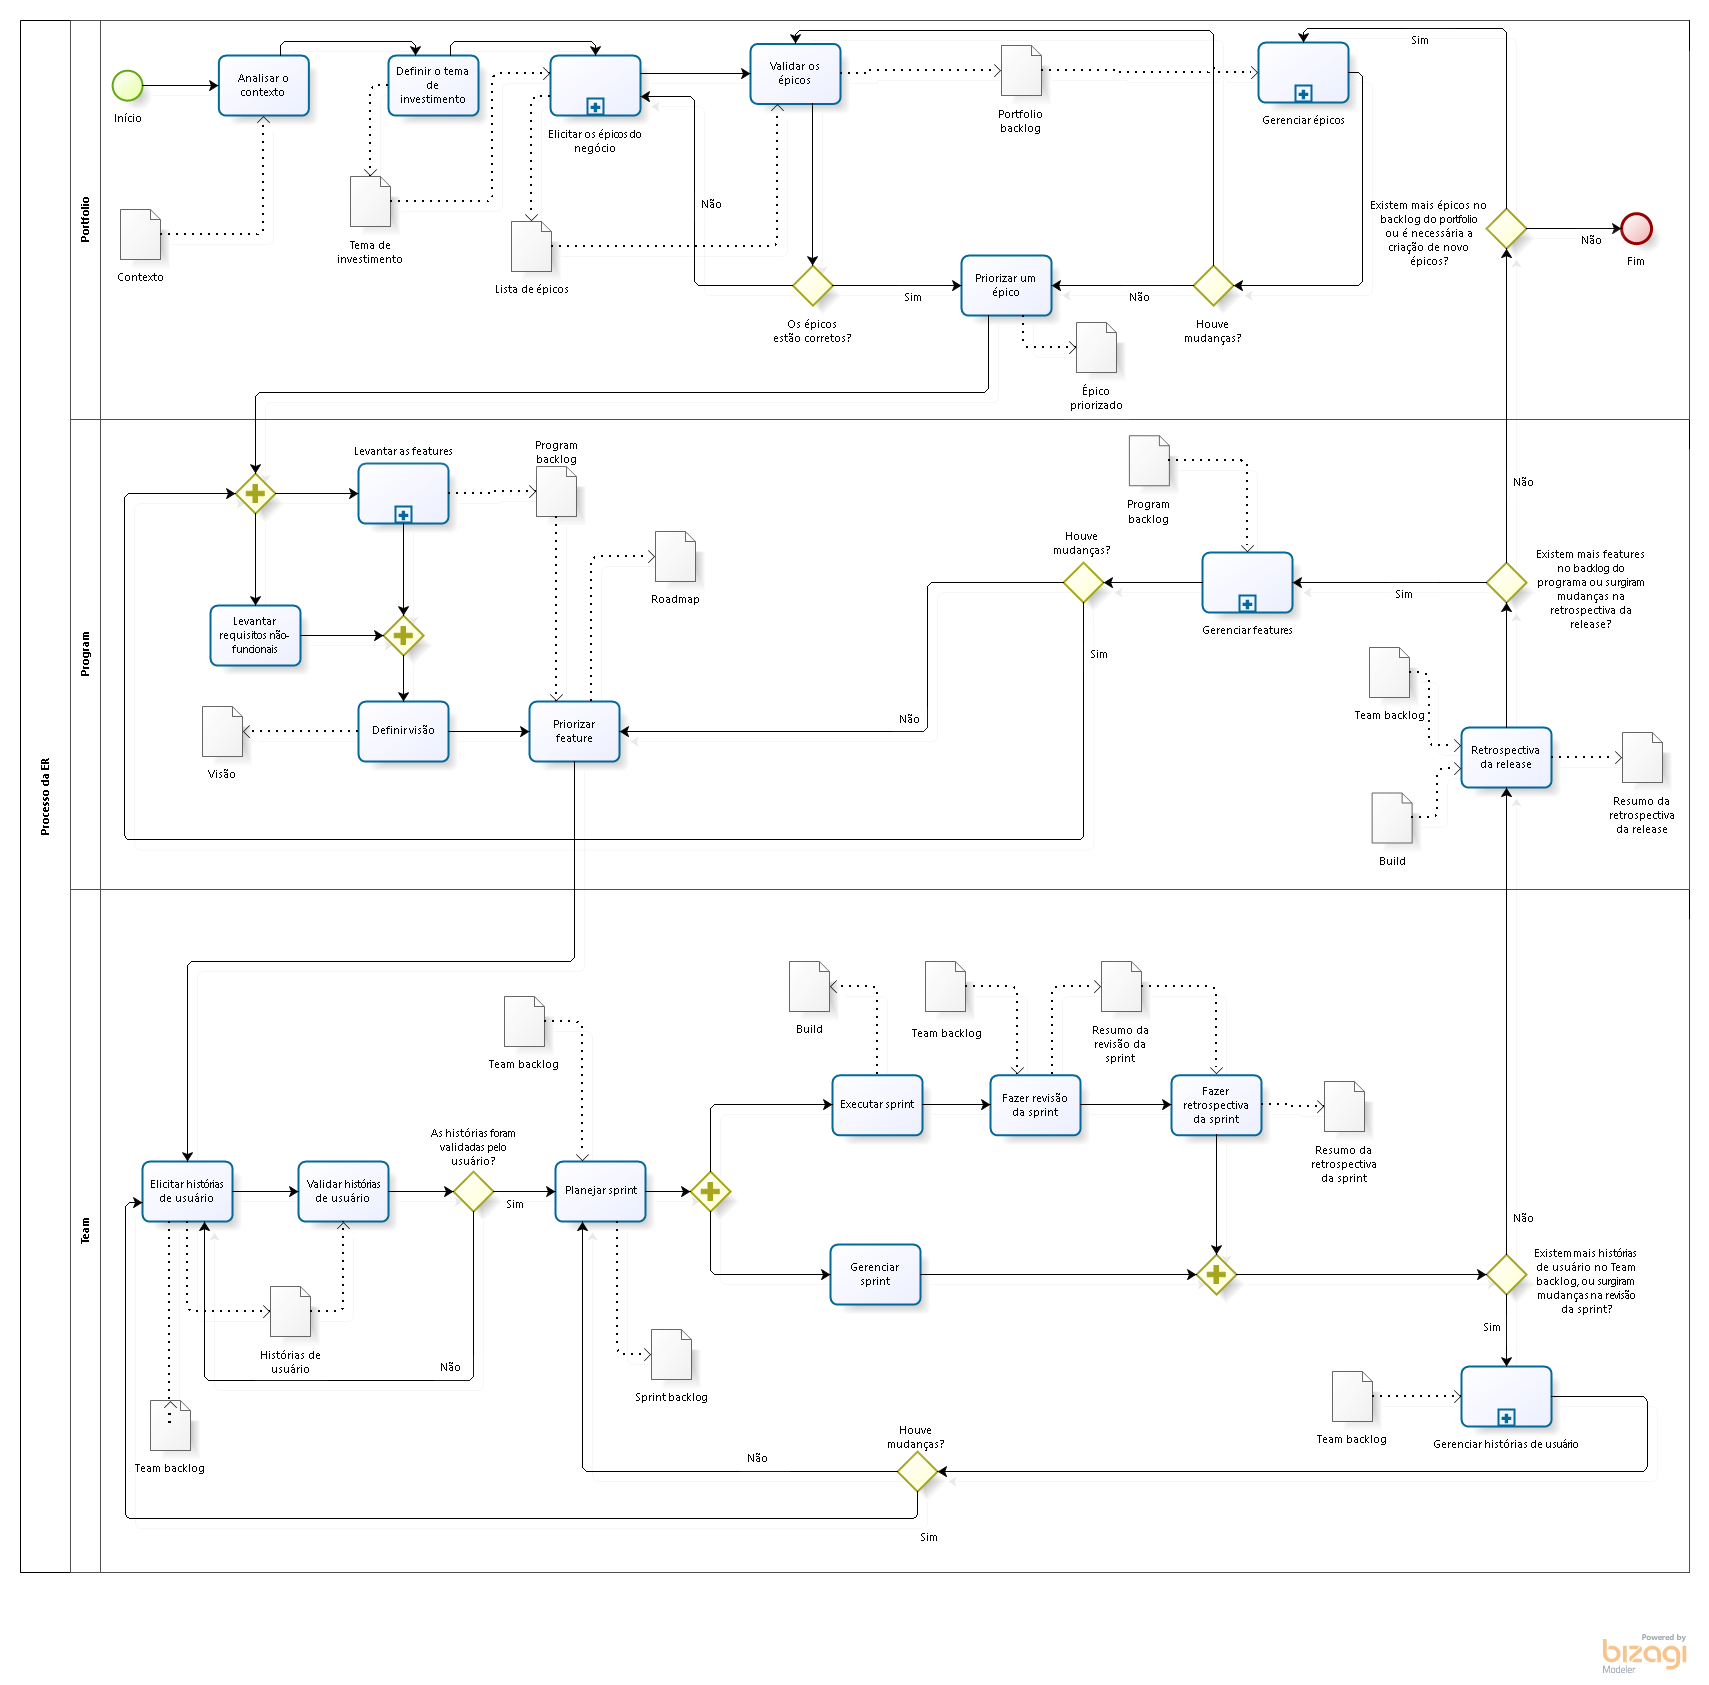
\includegraphics[scale=0.3]{figuras/Processo_v1-2}
    \caption[Big picture do processo.]{Big picture do processo. \footnotemark}
    \label{processo}
  \end{figure}

\section{Portfólio}
Esse nível tem como objetivo principal levantar e elaborar uma abstração de alto nível dos requisitos de negócio. Cada uma das atividades, artefatos gerados e papeis estabelecidos que serão descritos a seguir fazem parte da solução proposta para se resolver o problema existente. A execução de cada atividade será baseada na sistematização da análise documental e \textit{brainstormings}.

\subsection{Artefatos}
\begin{description}
\item[Contexto do cliente] É fornecido pelo cliente ou levantado a partir de outras fontes de informação que contenham dados sobre o próprio cliente e o problema a ser resolvido. Este artefato descreve resumidamente uma visão do contexto do problema e do cliente.
\item[Tema de investimento] Consiste na documentação de quais são os reais objetivos e valores da empresa e os benefícios que a solução em \textit{software} trará para a mesma. Por se tratar de um requisito de altíssimo nível é representado por uma breve descrição.
\item[Lista de Épicos] São iniciativas, ou frentes de negócio que podem gerar alto valor para o cliente, equipe ou o desenvolvimento de \textit{software} em si, como inovações arquiteturais ou implementação de tecnologias emergentes. Por se tratar de um requisito de alto nível, precisa ser trabalhado e refinado.
  \begin{enumerate}
    \item \textbf{Tempo:} um épico pode demandar tempo e vários ciclos de iteração para ser devidamente implementado.
    \item \textbf{Escopo:} por ser de alto nível afeta os subsequentes níveis do projeto, ocasionando um grande impacto e sendo uma área crítica pode custar muito para a equipe e cliente.
    \item \textbf{Negócio:} Representa a entrega de valor direta para o cliente, afetando diversos departamentos da área de negócios.
  \end{enumerate} 
\item[Backlog do Portfólio] Contém o detalhamento de cada um dos épicos e devidamente priorizados e organizados. Para isso, a cada épico é atribuida uma pontuação de acordo com sua complexidade seu valor gerado. Logicamente, para realizar uma avaliação precisa da complexidade da implementação do épico é necessário um detalhamento do mesmo.
\end{description}

\subsection{Descrição das atividades}

\newcolumntype{b}{>{\hsize=.7\hsize}X}
\newcolumntype{s}{>{\hsize=.3\hsize}X}

\begin{table}[!htbp]
\centering
\caption{Atividade: Analisar Contexto do Problema}
\label{atividade:1}
\begin{tabularx}{0.9\textwidth}{|>{\columncolor[HTML]{BBDAFF}}s |b|}
\hline
Identificador & 01                                                                  \\ \hline
Título        & Analisar contexto do problema                                       \\ \hline
Descrição     & Serão realizados encontros de forma que o cliente possa esclarecer o contexto no qual está inserido o problema, de forma que se busque um primeiro contato e o estabelecimento de um canal de diálogo da equipe com o cliente. \\ \hline
Entradas       & Contexto do Cliente                                                  \\ \hline
Saídas         & Temas de Investimentos                                               \\ \hline
Responsável   & Time                                                                  \\ \hline
\end{tabularx}
\end{table}

\begin{table}[!htbp]
\centering
\caption{Atividade: Definir tema de investimento}
\label{atividade:2}
\begin{tabularx}{0.9\textwidth}{|>{\columncolor[HTML]{BBDAFF}}s |b|}
\hline
Identificador & 02                                                                    \\ \hline
Título        & Definir tema de investimento                                          \\ \hline
Descrição     & Reunião entre o cliente e o gerente de portfolio a fim de definir o tema de investimento. \\ \hline
Entradas      &                                                                       \\ \hline
Saídas        & Tema(s) de investimento                                               \\ \hline
Responsável   & Gerente de portfolio                                                  \\ \hline
\end{tabularx}
\end{table}

\begin{table}[!htbp]
\centering
\caption{Atividade: Elicitar os épicos do negócio}
\label{atividade:3}
\begin{tabularx}{0.9\textwidth}{|>{\columncolor[HTML]{BBDAFF}}s |b|}
\hline
Identificador & 03                                                                    \\ \hline
Título          & Elicitar os épicos do negócio                                       \\ \hline
Descrição       & Criar uma lista de épicos pertinentes ao tema de investimento, isso poderá ser feito através de um brainstorm. \\ \hline
Entradas        & Tema de investimento                                                \\ \hline
Saídas        & Lista de épicos                                                       \\ \hline
Responsável   & Gerente de portfolio                                                  \\ \hline                                               
\end{tabularx}
\end{table}

\begin{table}[!htbp]
\centering
\caption{Atividade: Validar os épicos}
\label{atividade:4}
\begin{tabularx}{0.9\textwidth}{|>{\columncolor[HTML]{BBDAFF}}s |b|}
\hline
Identificador & 04                                                                    \\ \hline
Título          & Validar os épicos                                                   \\ \hline
Descrição       & Será realizada uma reunião entre o cliente e o gerente de portfolio com o objetivo de validar os épicos levantados. \\ \hline
Entradas        & Lista de épicos                                                     \\ \hline
Saídas          & Portfolio backlog                                                   \\ \hline
Responsável   & Gerente de portfolio                                                  \\ \hline
\end{tabularx}
\end{table}

\begin{table}[!htbp]
\centering
\caption{Atividade: Priorizar um épico}
\label{atividade:5}
\begin{tabularx}{0.9\textwidth}{|>{\columncolor[HTML]{BBDAFF}}s |b|}
\hline
Identificador & 05                                                                     \\ \hline
Título          & Priorizar um épico                                                   \\ \hline
Descrição      & O gerente de portfolio irá decidir em uma conversa com o cliente qual é o épico mais importante a ser realizado naquele momento do projeto.                                                                                    \\ \hline
Entradas      & Portfolio backlog                                                      \\ \hline
Saídas        & Épico priorizado                                                       \\ \hline
Responsável   & Gerente de portfolio                                                   \\ \hline
\end{tabularx}
\end{table}

\begin{table}[!htbp]
\centering
\caption{Atividade: Gerenciar os épicos}
\label{atividade:6}
\begin{tabularx}{0.9\textwidth}{|>{\columncolor[HTML]{BBDAFF}}s |b|}
\hline
Identificador & 06                                                                      \\ \hline
Título          & Gerenciar os épicos                                                   \\ \hline
Descrição      & O gerente de portfolio junto ao resto da equipe irão verificar se existem mais épicos no portfolio backlog ou se é necessária a criação de novos épicos.                                                                        \\ \hline
Entradas      & Portfolio backlog                                                       \\ \hline
Saídas        &                                                                         \\ \hline
Responsável   & Gerente de portfolio                                                    \\ \hline                                  
\end{tabularx}
\end{table}

\section{Programa}
Nessa etapa do processo se baseia na identificação de features e requisitos não-funcionais, na elaboração das correspondentes histórias de usuário e no planejamento das entregas do \textit{software}. Há também uma preocupação em se estabelecer estratégias para o desenvolvimento eficaz do \textit{software}.

\subsection{Artefatos}
\begin{description}
\item[Program Backlog] É o documento onde as \textit{features} são registradas, como uma pilha de \textit{features}.
\item[Roadmap] Consiste em uma série de \textit{releases} com datas planejadas, cada uma pertinente a um tema, um conjunto de objetivos e a priorização das \textit{features}. O \textit{Roadmap} nos dá uma ideia de como a equipe planeja mostrar valor no decorrer do tempo~\cite{leffingwell}.
\item[Visão] É um mecanismo utilizado para definir e comunicar diversos aspectos do sistema. Segundo Leffingwell~(\citeyear{leffingwell}), a visão de um sistema é composta por um conjunto de características que irão descrever as possibilidades do sistema, isto é, tudo aquilo que ele poderá oferecer ao usuário a fim de atender as necessidades dos envolvidos.
\end{description}

\clearpage

\subsection{Descrição das atividades}

\begin{table}[!htbp]
\centering
\caption{Atividade: Levantar \textit{features}}
\label{atividade:7}
\begin{tabularx}{0.9\textwidth}{|>{\columncolor[HTML]{BBDAFF}}s |b|}
\hline
Identificador & 07                                                                  \\ \hline
Título        & Levantar \textit{features}                                          \\ \hline
Descrição     & Consiste em levantar e detalhar a partir de técnicas conhecidas como reuniões e \textit{brainstormings} diversas funcionalidades que fazem parte do escopo do épico previamente selecionado.                                 \\ \hline
Entrada       & Épico da Iteração                                                   \\ \hline
Saída         & \textit{Program Backlog} e insumos para o Documento de Visão        \\ \hline
Responsável   & Time                                                                \\ \hline
\end{tabularx}
\end{table}

\begin{table}[!htbp]
\centering
\caption{Atividade: Levantar requisitos não-funcionais}
\label{atividade:8}
\begin{tabularx}{0.9\textwidth}{|>{\columncolor[HTML]{BBDAFF}}s |b|}
\hline
Identificador & 08                                                                   \\ \hline
Título        & Levantar requisitos não-funcionais                                  \\ \hline
Descrição     & A partir da realização de reuniões com os clientes e o time serão levantadas algumas condições para a construção da solução. Padrões de projeto, arquitetura, servidores, acessibilidade, etc.                               \\ \hline
Entrada       & \textit{Portfolio Backlog}                                          \\ \hline
Saída         & Insumos para o Documento de Visão                                   \\ \hline
Responsável   & Time                                                                \\ \hline
\end{tabularx}
\end{table}

\begin{table}[!htbp]
\centering
\caption{Atividade: Definir visão}
\label{atividade:9}
\begin{tabularx}{0.9\textwidth}{|>{\columncolor[HTML]{BBDAFF}}s |b|}
\hline
Identificador & 09                                                                   \\ \hline
Título        & Definir visão                                                       \\ \hline
Descrição     & A partir dos insumos fornecidos pelas diversas reuniões e de um pensamento alinhado da equipe e cliente sobre o problema a ser resolvido,será elaborado um documento que contenha os fatores e os pontos de discussão mais relevantes para a concepção e construção do \textit{software}.                                                                                              \\ \hline
Entrada       & \textit{Backlog do Programa}                                        \\ \hline
Saída         & Documento de Visão                                                  \\ \hline
Responsável   & Time                                                                \\ \hline
\end{tabularx}
\end{table}

\clearpage

\begin{table}[!htbp]
\centering
\caption{Atividade: Priorizar \textit{features}}
\label{atividade:10}
\begin{tabularx}{0.9\textwidth}{|>{\columncolor[HTML]{BBDAFF}}s |b|}
\hline
Identificador & 10                                                                  \\ \hline
Título        & Priorizar \textit{features}                                         \\ \hline
Descrição     & Com as \textit{features} definidas, cada uma deve receber uma pontuação de acordo com sua relevância, ou seja, valor que agrega para o cliente e dificuldade de implementação.                                                \\ \hline
Entrada       & \textit{Backlog do Programa}                                        \\ \hline
Saída         & \textit{Roadmap}                                                    \\ \hline
Responsável   & Time                                                                \\ \hline
\end{tabularx}
\end{table}

\begin{table}[!htbp]
\centering
\caption{Atividade: Gerenciar \textit{features}}
\label{atividade:11}
\begin{tabularx}{0.9\textwidth}{|>{\columncolor[HTML]{BBDAFF}}s |b|}
\hline
Identificador & 11                                                                   \\ \hline
Título        & Gerenciar \textit{features}                                          \\ \hline
Descrição     & A cada nova release são levantadas novas features para serem divididas em conjuntos de histórias de usuário, esta atividade tem por objetivo refinar as features para se adequarem às novas necessidades dos \textit{stakeholders}.                                        \\ \hline
Entrada       & \textit{Backlog} do Programa e possíveis novas features              \\ \hline
Saída         & Refinamento das \textit{features}                                    \\ \hline
Responsável   & Time                                                                 \\ \hline
\end{tabularx}
\end{table}

\begin{table}[!htbp]
\centering
\caption{Atividade: Retrospectiva da \textit{Release}}
\label{atividade:12}
\begin{tabularx}{0.9\textwidth}{|>{\columncolor[HTML]{BBDAFF}}s |b|}
\hline
Identificador & 12                                                                   \\ \hline
Título        & Retrospectiva da \textit{Release}                                    \\ \hline
Descrição     & Tem como objetivo validar o que foi produzido na release, juntamente com os envolvidos, a Retrospectiva da \textit{Release} ocorre depois da Revisão da Sprint, caso não existam mais mudanças desejadas e todas as histórias de usuário estejam completas.                \\ \hline
Entrada       & \textit{Backlog} do Time e a \textit{Release} atual do sistema       \\ \hline
Saída         & Resumo da retrospectiva da \textit{Release}                          \\ \hline
Responsável   & Time                                                                 \\ \hline
\end{tabularx}
\end{table}

\section{Time}
O nível da equipe descreve como as equipes ágeis aplicam o SAFe integrado com as práticas Scrum/XP e análise de qualidade para garantir a entrega da solução descrita nos documentos de requisitos.

\subsection{Artefatos}
\begin{description}
\item[Team Backlog] Representa uma coleção de tudo que o time necessita para implementar aquela parte do sistema. Pode conter histórias de usuário ou \textit{enabler histories}. Sendo que a maioria tem origem no \textit{Program Backlog}, enquanto algumas são pertinentes a um contexto específico do time. O \textit{Team Backlog} pertence ao P.O., vale salientar que o fato de "pertencer" ao P.O. não significa que ele é o único que pode alterá-lo, mas é preferível que seja ele a fazer isso. (REFERÊNCIA SAFe, 2015)
\item[Sprint Backlog] É uma lista de tarefas que o time se compromete a fazer em uma \textit{sprint}. Os itens do \textit{Sprint Backlog} são extraídos do \textit{Team Backlog}, com base nas prioridades previamente definidas. É a percepção da equipe sobre o tempo que será necessário para completar um conjunto de funcionalidades.
\item[Build] É o incremento gerado a cada \textit{sprint}.
\end{description}

\clearpage

\subsection{Descrição das atividades}

\begin{table}[!htbp]
\centering
\caption{Atividade: Elicitar histórias de usuário}
\label{atividade:13}
\begin{tabularx}{0.9\textwidth}{|>{\columncolor[HTML]{BBDAFF}}s |b|}
\hline
Identificador & 13                                                                   \\ \hline
Título        & Elicitar histórias de usuário                                         \\ \hline
Descrição     & A partir do \textit{Backlog} do Time, esta atividade tem por objetivo levantar as histórias de usuário em conjunto com os \textit{stakeholders}, utilizando as técnicas de elicitação definidas, a partir das \textit{features} escolhidas para serem implementadas durante a \textit{sprint}.                                                                     \\ \hline
Entrada       & \textit{Backlog} do Time e \textit{Roadmap}    		                \\ \hline
Saída         & Histórias de usuário                                                 \\ \hline
Responsável   & Time                                                                 \\ \hline
\end{tabularx}
\end{table}

\begin{table}[!htbp]
\centering
\caption{Atividade: Validar histórias de usuário}
\label{atividade:14}
\begin{tabularx}{0.9\textwidth}{|>{\columncolor[HTML]{BBDAFF}}s |b|}
\hline
Identificador & 14                                                                   \\ \hline
Título        & Validar histórias de usuário                                         \\ \hline
Descrição     & Consiste em validar as histórias de usuário elicitadas em conjunto com os \textit{stakeholders}.                                                               \\ \hline
Entrada       & Histórias de usuário       							                \\ \hline
Saída         & Validação das histórias de usuário e insumos para o planejamento da sprint                          \\ \hline
Responsável   & Time                                                                 \\ \hline
\end{tabularx}
\end{table}

\begin{table}[!htbp]
\centering
\caption{Atividade: Planejar \textit{sprint}}
\label{atividade:15}
\begin{tabularx}{0.9\textwidth}{|>{\columncolor[HTML]{BBDAFF}}s |b|}
\hline
Identificador & 15                                                                  \\ \hline
Título        & Planejar \textit{sprint}                                            \\ \hline
Descrição     & Após análise de cada item do \textit{Team Backlog}, o time estima o esforço necessário para a realização de cada item. Então sabendo o que é prioritário para o \textit{Product Owner}, define-se o que será realizado na \textit{sprint} em questão, formando o \textit{Sprint Backlog}.\\ \hline
Entrada       & \textit{Team Backlog}                                               \\ \hline
Saída         & \textit{Sprint Backlog}                                             \\ \hline
Responsável   & \textit{Scrum Master}, Time                                         \\ \hline
\end{tabularx}
\end{table}

\begin{table}[!htbp]
\centering
\caption{Atividade: Executar \textit{sprint}}
\label{atividade:16}
\begin{tabularx}{0.9\textwidth}{|>{\columncolor[HTML]{BBDAFF}}s |b|}
\hline
Identificador & 16                                                                  \\ \hline
Título        & Executar \textit{sprint}                                            \\ \hline
Descrição     & Representa um ciclo de trabalho. As \textit{sprints} devem ter sempre a mesma duração, uma semana.” A cada \textit{sprint} um conjunto de requisitos é implementado, tendo como resultado um incremento do produto que está sendo desenvolvido.\\ \hline
Entrada       & \textit{Sprint Backlog}                                             \\ \hline
Saída         & \textit{Build}                                                      \\ \hline
Responsável   & Time                                                                \\ \hline
\end{tabularx}
\end{table}

\begin{table}[!htbp]
\centering
\caption{Atividade: Fazer revisão da \textit{sprint}}
\label{atividade:17}
\begin{tabularx}{0.9\textwidth}{|>{\columncolor[HTML]{BBDAFF}}s |b|}
\hline
Identificador & 17                                                                  \\ \hline
Título        & Fazer revisão da \textit{sprint}                                    \\ \hline
Descrição     & Aqui é revisado com o Product owner o que foi gerado ao produto após a execução da sprint. Os itens do Sprint Backlog que não foram gerados são adiados para a próxima sprint.                                               \\ \hline
Entrada       & \textit{Team Backlog}                                               \\ \hline
Saída         & Resumo da revisão da \textit{sprint}                                \\ \hline
Responsável   & Time, \textit{Scrum Master}, \textit{Product Owner}                 \\ \hline
\end{tabularx}
\end{table}

\begin{table}[!htbp]
\centering
\caption{Atividade: Fazer retrospectiva da \textit{sprint}}
\label{atividade:18}
\begin{tabularx}{0.9\textwidth}{|>{\columncolor[HTML]{BBDAFF}}s |b|}
\hline
Identificador & 18                                                                  \\ \hline
Título        & Fazer revisão da \textit{sprint}                                    \\ \hline
Descrição     & Nesta atividade, a equipe se reúne para levantar as práticas que deram certo na \textit{sprint}, o que deu errado, e o que pode ser feito para melhorar.                                                                     \\ \hline
Entrada       & Resumo da Revisão da \textit{sprint}                                \\ \hline
Saída         & Resumo da Retrospectiva da \textit{sprint}                          \\ \hline
Responsável   & Time, \textit{Scrum Master}                                         \\ \hline
\end{tabularx}
\end{table}

\begin{table}[!htbp]
\centering
\caption{Atividade: Gerenciar \textit{sprint}}
\label{atividade:19}
\begin{tabularx}{0.9\textwidth}{|>{\columncolor[HTML]{BBDAFF}}s |b|}
\hline
Identificador & 19                                                                   \\ \hline
Título        & Gerenciar \textit{sprint}                                            \\ \hline
Descrição     & Tem por objetivo gerenciar o desenvolvimento e possíveis mudanças, além de acompanhar e dar suporte ao time durante a \textit{sprint}.                          \\ \hline
Entrada       & \textit{Backlog da Sprint}       							        \\ \hline
Saída         &                                                                       \\ \hline
Responsável   & Time                                                                  \\ \hline
\end{tabularx}
\end{table}

\begin{table}[!htbp]
\centering
\caption{Atividade: Gerenciar histórias de usuário}
\label{atividade:20}
\begin{tabularx}{0.9\textwidth}{|>{\columncolor[HTML]{BBDAFF}}s |b|}
\hline
Identificador & 20                                                                   \\ \hline
Título        & Gerenciar histórias de usuário                                       \\ \hline
Descrição     & Tem os objetivos de acompanhar o \textit{Backlog} do Time, verificar possíveis mudanças nas histórias de usuário e analisar os impactos causados por essas possíveis mudanças.                                                                    \\ \hline
Entrada       & \textit{Backlog} do Time e possíveis novas histórias de usuário      \\ \hline
Saída         & \textit{Backlog} do Time atualizado                        		    \\ \hline
Responsável   & Time                                                                 \\ \hline
\end{tabularx}
\end{table}
